\section{Approach}
\label{sec:approach}

\name follows the pipeline shown in \autoref{fig:pipeline}. Given a domain specification and a small set of generation controls, \name constructs benchmark instances in four stages: 
(i) it generates a \emph{latent relational source} (\S\ref{subsec:data-generation}); 
(ii) it applies executable SQL programs and computes their gold answers (\S\ref{subsec:sql-execution}); 
(iii) it renders the latent source as one or more perturbed \emph{non-relational views}, preserving answer correctness through provenance masks (\S\ref{subsec:transformations});
and (iv) it verbalizes the SQL programs into NL questions (\S\ref{subsec:nl-generation}). The generated NL questions and non-relational views are used for model evaluation.
%The latent relational source is used only inside \name for supervision and verification, with the evaluated LLM receiving only the non-relational views and the natural-language question. This separation lets us vary table layout, noise, units, and multi-table reasoning structure without changing the gold answer.

\subsection{Latent Relational Source Generation}
\label{subsec:data-generation}


% The generated schema includes the table name, attribute names, human-readable headers \mpaga{qual è la differenza con attribute names?} \mlc{più verbosi, non camel case ecc.}, attribute types, candidate value ranges, one distinguished numerical value attribute \mpaga{perché uno? l'utente può richiedere che la tabella sia costituita da più campi numerici? Se no, come mi sembra di aver capito, non richiamo di generare tabelle poco realistiche? Come ci difendiamo? Non possiamo dire che in questo step l'utente specifica i suoi desiderata con eventualmente anche molteplici colonne numeriche, ma poi noi internamente ad un certo punto siamo obbligati a selezionarne uno} \mlc{il limite è a livello di perturbazione: il pivot si può fare solamente con un attributo numerico. Siccome stiamo generando da LLM, gli chiediamo direttamente di generarne uno, e non tanti, in quanto i restanti attributi verrebbero scartati. Nello scenario con tabelle reali, invece, selezioniamo quelle tabelle che hanno almeno un attributo float, e poi ne selezioniamo uno tra quelli come hai detto \autoref{fig:real_table_feasibility}. La realisticità delle tabelle non è un obiettivo, in quanto il setting "from-scratch" è altamente complesso, ma l'obiettivo è quello di dire che per certe domande la performance è molto bassa, che le domande sono rispondibili (anche se non sono 100\% vere), e che allenare sulle tabelle generate da noi ha dei benefici (vedere risultati). Forse dovremmo indicare subito nel paper che il nostro claim non è quello di generare tabelle realistiche}, and metadata about units of measurement and decimal precision.

% To steer generation toward realistic domains, we optionally condition the prompt on example tables and on domain-specific inventories of canonical units.
% Concretely, \name\ uses conversion resources derived from the Quantities, Units, Dimensions and Types ontology (QUDT)~\cite{qudt} for environmental quantities and the XBRL Units Registry (XBRL UTR)~\cite{xbrlutr} for finance.
%This stage constructs the latent relational source in two steps. First, \name prompts an LLM to generate a domain-specific schema, conditioned on a user-defined target domain, attribute count, attribute cardinalities, and previously generated table names. This encourages related but non-identical tables. \mlc{to say that the previous table names is not defined by the user, but based on previous interactions} The schema specifies the table name, attributes with types and candidate values, unit and decimal precision metadata, and a designated numerical attribute for quantitative reasoning.
This stage constructs the latent relational source in two steps. First, \name prompts an LLM to generate a domain-specific schema, conditioned on a user-defined target domain, attribute count, and attribute cardinalities, together with the names of previously generated tables, which are supplied automatically by the system from prior generation steps. This encourages related but non-identical tables. The schema specifies the table name; the attributes, each with its type and a corresponding value range; unit metadata; and a designated numerical attribute for quantitative reasoning.
To steer generation toward realistic domains, the prompt can be grounded in example tables and domain-specific unit inventories, such as the Quantities, Units, Dimensions and Types ontology (QUDT)~\cite{qudt} for environmental data and the XBRL Units Registry (XBRL UTR)~\cite{xbrlutr} for financial data.

Second, \name instantiates the schema as a dense latent relational source by enumerating combinations of categorical attributes and sampling the numerical field. During instantiation, it enforces lightweight semantic regularities, including column dependencies (e.g., city $\longrightarrow$ country) and cross-row numerical constraints (e.g., a ``gross'' value exceeds its corresponding ``net'' value for the same entity and period). We defer their formalization and solver implementation to \S\ref{sec:semantic_constraints}. 

The resulting latent relational source serves as the unified basis for SQL supervision, question generation, and the construction of multiple non-relational views. Rather than generating these views independently, \name derives them from the same latent representation through table-specific projections and transformations. %This preserves ground-truth correspondences across views while enabling controlled reasoning topologies and automatically verifiable answers.

\eat{
\name begins by prompting an LLM to generate a plausible domain-specific schema, conditioned on the target domain, the desired number of attributes, the attribute cardinalities, and the history of previously generated table names, which encourages the LLM to produce related but non-identical tables.
The resulting schema specifies the table name, a set of attributes with their types and candidate value ranges, metadata on units of measurement and precision, and includes a designated numerical attribute that will later support quantitative reasoning.

To steer generation toward realistic domains, the prompt can be grounded in example tables and domain-specific unit inventories, such as the Quantities, Units, Dimensions and Types ontology (QUDT)~\cite{qudt} for environmental data and the XBRL Units Registry (XBRL UTR)~\cite{xbrlutr} for financial data.


Given the schema, \name\ instantiates a dense latent relational source by enumerating combinations of categorical attributes and sampling values from the numerical field. 
During this process, it enforces lightweight semantic regularities to increase realism, including column dependencies (e.g., city $\longrightarrow$ country) and cross-row numerical consistency constraints (e.g., a “gross” value is always greater than its corresponding “net” value for the same entity and time period). We defer the formalization and solver implementation of these constraints to \S\ref{sec:semantic_constraints}. 

The resulting latent relational source serves as the unified basis for SQL supervision, question generation, and the construction of multiple non-relational views.
Rather than generating these views independently, \name\ derives them from the same latent representation through table-specific projections and transformations. This preserves a known ground-truth correspondence between evidence pieces across views while enabling controlled reasoning topologies and automatically verifiable answers.}
%The resulting latent relational source serves as the unified basis for SQL supervision, question generation, and subsequent view construction.
% To improve plausibility, the generator also samples lightweight semantic regularities over the table and enforces them during instantiation; these include row-level implications and cross-row numerical consistency conditions \mpaga{Riporterei un esempio altrimenti non si capisce} \mlc{io non saprei neanche se dirlo questo in realtà, in quanto non ne discutiamo nel resto del paper. Rimanderei all'appendice: l'idea è che noi forniamo un sistema di generazione di constraint, non lo testiamo, ma un utente può semi-automaticamente usare questo sistema per cercare di creare tabelle più veritiere.}. We defer their exact formalization and solver implementation to \S\ref{sec:semantic_constraints}. The resulting latent relational source is the common basis for SQL supervision, question generation, and non-relational view rendering.
% For multi-table generation, \name\ does not sample unrelated sources independently. Instead, it derives multiple table-specific subsets from the same latent relational source, which are later rendered as non-relational views. This choice is important for two reasons. First, it preserves a known ground-truth correspondence between evidence pieces across views. Second, it allows us to control the reasoning topology and depth while keeping the final answer automatically verifiable.


\subsection{SQL Supervision and Multi-Table Reasoning}
\label{subsec:sql-execution}



% In the \textbf{parallel} setting, \name\ first samples a predicate template over a subset of categorical attributes that uniquely identifies one numerical value. \mpaga{Non possiamo fare riferimento alla figura per rendere il tutto più esemplificativo? Qui si riporta un esempio di predicato. Per esempio in tabella della figura applicare un predicato su azienda e settore è sufficiente per identificare un valore unico} Then it instantiates multiple table-specific selections by varying exactly one attribute across tables while keeping the remaining predicate structure fixed. \mpaga{Qui si fa riferimento al fatto che si mantiene fisso il settore} 
% From the latent relational source, \name\ applies executable SQL programs that define the target answer. SQL is used as an internal supervision language: programs are executed on the latent source to compute gold labels, while models receive only the non-relational views and the natural-language question. We focus on aggregation-style questions whose final answer is produced by combining different scalar values. 

% In the \textbf{parallel} setting, \name constructs a predicate over categorical attributes that isolates a target numerical value (e.g., company–sector pairs for a performance metric). Multiple views are then created by holding all conditions fixed except one varying attribute across tables (e.g., keeping the sector fixed while changing the company; see \autoref{fig:pipeline} \textcircled{2}).
% Each table-specific view contributes one scalar value $a_i$, and the final answer is computed by an aggregation operator
% \begin{equation}\label{eq:1}
% \begin{aligned}
% y &= g(a_1,\dots,a_n),\\
% g &\in \{\textsc{sum}, \textsc{avg}, \textsc{max}, \textsc{min}\}.
% \end{aligned}
% \end{equation}

This stage uses SQL as supervision: \name executes SQL queries over the latent relational source to compute gold labels. We focus on aggregation-style questions that combine scalar values.
% In the \textbf{parallel} setting, \name constructs a predicate over categorical attributes that isolates a target numerical value. It then creates multiple views by keeping the predicate fixed except for one attribute that varies across views (e.g., keeping the sector fixed while changing the company; see \autoref{fig:pipeline} \textcircled{2}). Each table-specific view contributes one scalar value $a_i$, and the final answer is computed as
% \begin{equation}\label{eq:1}
% \begin{aligned}
% y &= g(a_1,\dots,a_n),\\
% g &\in \{\mathrm{sum}, \mathrm{avg}, \max, \min\}.
% \end{aligned}
% \end{equation}

% Operationally, each view is associated with an extractive SQL query returning a single value, and the final label is obtained by applying the aggregation over the list of extracted scalars.  This is the mechanism used to create multi-table sum, average, and superlative questions.

In the \emph{parallel} setting, \name constructs a predicate over categorical attributes that isolates a target numerical value. It instantiates multiple table-specific selections by keeping the predicate fixed except for one attribute that varies across views (e.g., keeping the sector fixed while changing the company; see \autoref{fig:pipeline}). %\textcircled{2}).
Each view contributes one scalar $a_i$, and the final answer is computed as $y=g(a_1,\dots,a_n)$, with $g \in \{\mathrm{sum}, \mathrm{avg}, \max, \min\}$. Thus, parallel instances correspond to multi-table \emph{quantitative} (sum, average), and \emph{comparative} questions (superlative operations like max, min), with one extractive SQL query per view and one aggregation over the scalars.

% In the \textbf{sequential} setting, \name\ constructs a chain of table-local queries. Intermediate views are associated with extractive queries whose returned value becomes the lookup key for the next view in the chain, while the final view applies the target numerical aggregation. Formally, if $b_1$ is extracted from $T_1$, then $b_1$ parameterizes the selection on $T_2$, whose output parameterizes the next step, and so on until the last view produces the values needed for the final aggregation. \mpaga{Sostituirei la frase precedente con un riferimento all'esempio di Figura per spiegare la catena} The final aggregation uses the same operators as in \autoref{eq:1}, applied to a randomly sampled set of 2 to 5 values returned by the last view. The gold label is the result of executing this latent composition. This setup yields multi-step reasoning across tables without relying on an externally given relational schema.

In the \emph{sequential} setting, \name\ constructs a chain of table-local queries. Intermediate views are associated with extractive queries whose returned value becomes the only lookup key for the next view in the chain, while the final view applies the target numerical aggregation. The final aggregation uses the same operators as in the parallel setting, applied to a randomly sampled set of 2 to 5 values returned by the last view. The gold label is the result of executing this latent composition. This setup yields multi-step reasoning across tables without relying on an externally given relational schema. For instance, the example in \autoref{fig:pipeline} requires identifying the company associated with John Doe, using that company to retrieve the AI and financial-sector investment values, and averaging them.

%Because all SQL programs are executed on the latent relational source before view rendering and perturbation, answer correctness is guaranteed by construction. Moreover, since the same latent source can be reused to generate multiple types of questions and different numbers of views, the approach scales naturally between reasoning depths and evidence cardinalities.
Since the same latent source can be reused to generate multiple types of questions and different numbers of views, the approach scales naturally between reasoning depths and evidence cardinalities.

\begin{figure*}[t!]
    \centering

    \begin{subfigure}[t]{0.32\textwidth}
        \centering
        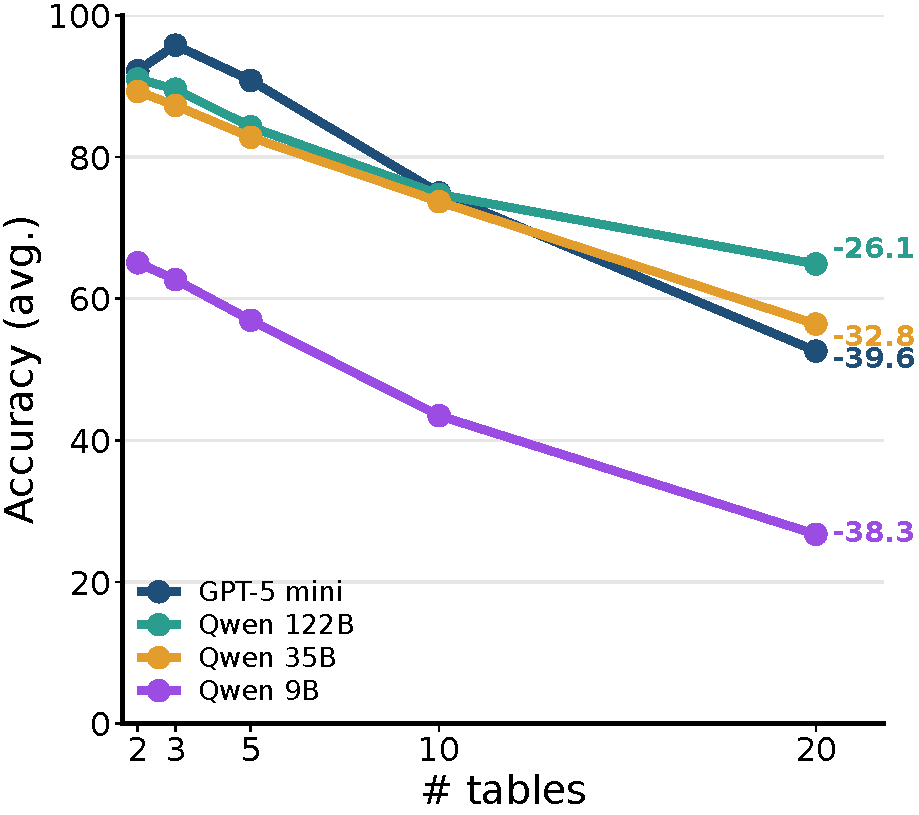
\includegraphics[width=\linewidth]{img/scaling_parallel.pdf}
        \caption{Parallel questions}
        \label{fig:parallel_scaling}
    \end{subfigure}
    \hfill
    \begin{subfigure}[t]{0.32\textwidth}
        \centering
        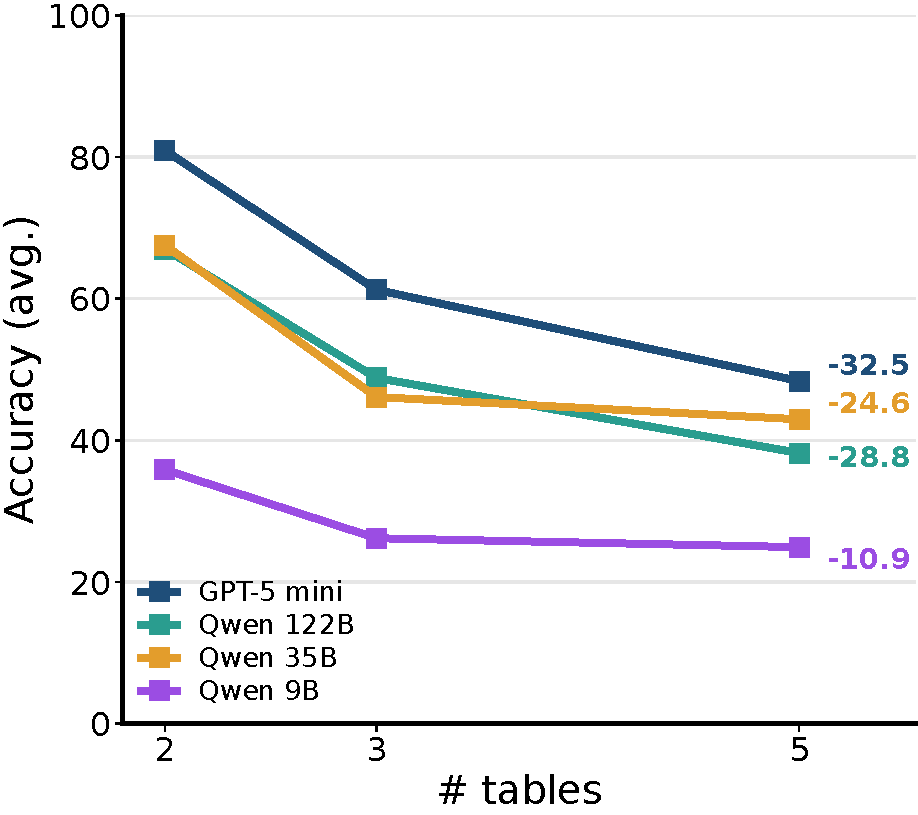
\includegraphics[width=\linewidth]{img/scaling_sequential.pdf}
        \caption{Sequential questions}
        \label{fig:sequential_scaling}
    \end{subfigure}
    \hfill
    \begin{subfigure}[t]{0.32\textwidth}
        \centering
        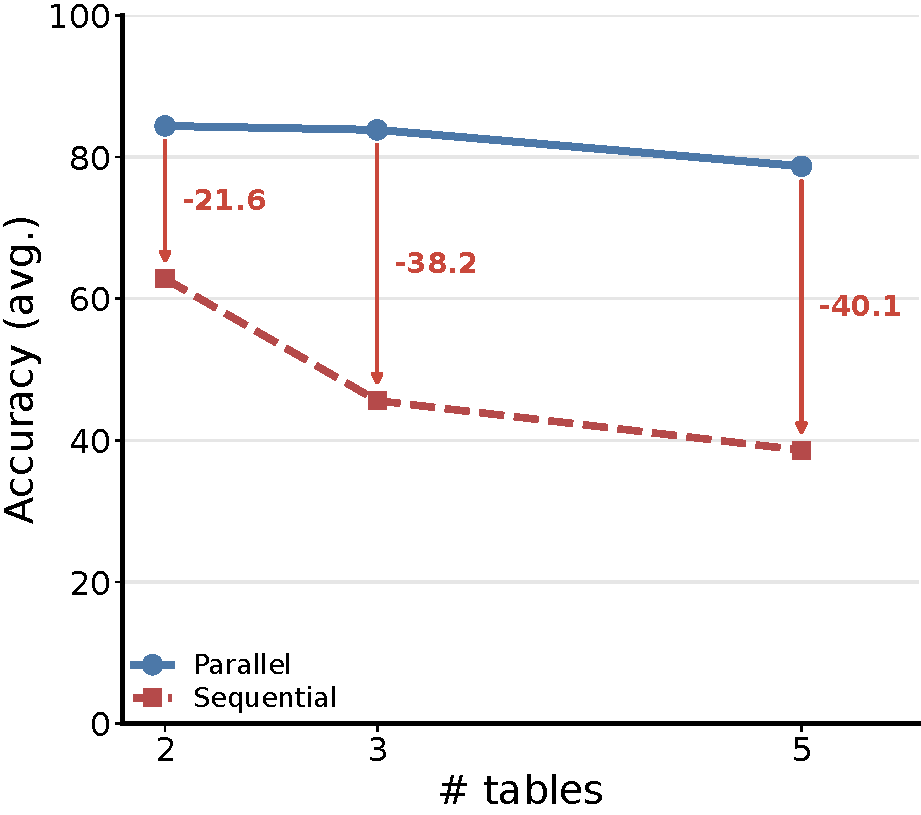
\includegraphics[width=\linewidth]{img/par_vs_seq.pdf}
        \caption{Parallel vs sequential}
        \label{fig:parallel_sequential_penalty}
    \end{subfigure}

    % \caption{
    % Scaling behavior as the number of tables increases.
    % The numbers at the end of each model curve in (a) and (b) report the accuracy drop from the smallest to the largest evaluated number of tables.
    % Panel (c) compares the average performance of parallel and sequential questions at the same table counts, showing that sequential reasoning introduces an additional degradation beyond multi-table aggregation alone.
    % }
    \caption{
    Scaling behavior as the number of tables increases.
    Labels at the end of curves in (a) and (b) report the accuracy drop from the smallest to largest table count.
    Panel (c) compares parallel and sequential questions at matched table counts, showing that sequential reasoning adds degradation beyond multi-table aggregation.
}
    \label{fig:scaling_parallel_sequential}
\end{figure*}

\subsection{Rendering Non-Relational Views}
\label{subsec:transformations}

Rendering is organized as an answer-preserving transformation sequence. \name first creates table-specific relational projections from the latent source and records a provenance mask marking cells required by the SQL program and cells safe to perturb. It then introduces null values, and applies column merging, unit rendering and conversion while the representation is still relational. Next, \name converts each projection into a non-relational view through a pivot-style transformation, organizing selected attributes as hierarchical row and column headers. The generator searches over candidate row/column partitions, prefers dense pivots, shrinks the layout, and retains all evidence required by the SQL program. Rendered views are capped at a user-specified size. After layout construction, \name inserts perturbations such as blank rows or columns, typographical noise, and contextual or footnote-like text.

The same rendering machinery supports both multi-table regimes, with scenario-specific controls. In parallel generation, each view provides one independently retrievable scalar for the final aggregation, and unit conversion can force normalization across compatible quantities. In sequential generation, each view represents one step of a latent lookup chain. Intermediate views contain exactly one occurrence of the lookup key extracted from the previous view. This is an evaluation choice rather than a framework limitation: ambiguous or tree-shaped joins would add uncontrolled variation in join complexity and the number of values entering the final aggregation. Unique matches keep the reasoning depth comparable across instances while still requiring models to recover implicit cross-table links, since latent joins are not stated in the question. Finally, view order is randomized to prevent shortcutting. 
% Overall, rendering produces non-relational views that hide clean schemas, explicit joins, and standardized numerical expressions but remain verifiable through the latent relational source and SQL supervision.
Overall, rendering hides clean schemas, explicit joins, and standardized numerical expressions while preserving verifiability through the latent relational source and SQL supervision.

\eat{
\fg{To construct the input given to the evaluated LLM, \name renders the latent relational source as non-relational views.} These transformations are answer-preserving: \name tracks the cells required by the SQL program and prevents perturbations from deleting or corrupting the evidence needed to recover the gold label.

We first apply schema-level changes, such as replacing synthetic attribute names with longer web-style headers and optionally merging columns. We then render measurement units either in headers or directly inside cells. Next, we convert flat tables into non-relational layouts through a pivot-style transformation that organizes selected attributes as hierarchical row and column headers. The generator searches over candidate row/column partitions, prefers dense pivots, and shrinks the resulting layout while ensuring that all evidence cells required by the latent SQL program are retained. \fg{In all experiments, rendered views are capped at $10 \times 10$ cells to keep inputs compact.} This is the main mechanism by which \name produces nested headers and non-trivial table layouts.

%\fg{If a perturbation would remove or corrupt an answer-bearing cell, \name{} restores the required evidence before finalizing the view.}

%The same transformation machinery is used for both multi-table regimes, but the source-to-\fg{view} mapping differs. In the parallel setting, each \fg{non-relational view} contains one independently retrievable scalar contribution to the final aggregation. In the sequential setting, each \fg{non-relational view} contains one step of a latent lookup chain, so that solving the question requires propagating information across \fg{views} before computing the final answer. In addition, for parallel generation \name\ can optionally apply unit conversion to some \fg{views} before perturbation, forcing models to normalize compatible quantities across heterogeneous surface forms. The converted values are accepted only when round-trip consistency can be maintained at the chosen decimal precision.



After layout construction, we apply cell- and structure-level perturbations, including blank rows and columns, null-like fillers in non-answer cells, typographical noise, and contextual or footnote-like text inserted into cells.  The same transformation machinery is used for both multi-table regimes, with additional scenario-specific controls.
For parallel generation, each non-relational view contains one independently retrievable scalar contribution to the final aggregation. Moreover, \name\ can optionally convert units inside each tabular view, forcing models to normalize compatible quantities across heterogeneous surface forms.
%Converted values are retained only when round-trip consistency can be preserved at the chosen decimal precision.

For sequential generation, each non-relational view contains one step of a latent lookup chain, so that solving the question requires propagating information across views before computing the final answer. Moreover, we constrain each intermediate view to contain exactly one occurrence of the lookup key extracted from the previous view.
This is an evaluation choice rather than a framework limitation: ambiguous or tree-shaped joins would introduce uncontrolled variation in both join complexity and the number of values entering the final aggregation.
By enforcing unique intermediate matches, we keep the reasoning depth comparable across instances while still requiring models to recover implicit cross-table links, since the latent joins are not stated in the question.
Finally, we randomize the order of sequential views to prevent models from using input order as a shortcut for the lookup chain.

Overall, this transformation stage yields benchmark instances that no longer expose a clean relational schema, explicit joins, or standardized numerical expressions, while still remaining fully verifiable. %because every question is grounded in a \fg{latent relational source} and an executable supervision program. %Additional details on perturbation types, constraint handling, and implementation choices are provided in the appendix.
\mpaga{La parte precedente non può essere riscritta con il seguente ordine o è necessaria una precedenza tra le trasformazioni, adesso mi sembra un po' confusionaria? 1) Pivoting, 2) Trasformazioni allo schema (sinonimi e merging), 3) Trasformazioni sui valori: noise sui valori (null, typos, inline text) + conversione dei valori (w.r.t. meas. unit), 4) constraint enforcing (solo per sequential)} \mlc{non è reso esplicito, ma dal punto di vista implementativo applichiamo alcune trasformazioni sulla view relazionale per: proteggerci da eventuali perturbazioni lossy (e.g. l'introduzione dei nan richiede una mask sulla tabella relazionale che ci indichi quali celle possiamo rendere nan), impossibilità di perturbazioni post-pivot (column merging sarebbe difficile, in quanto non sapremmo bene come unire righe che possono variare su molteplici livelli di header di riga/colonna: è più semplice farlo su tab. relazionale. Stessa cosa per unità di misura, a cui inoltre inseriamo l'unità di misura in maniere diverse: nelle celle, nell'header di colonna, in una cella in alto a sinistra nella tabella). Altre perturbazioni più semplici e locali (e.g. typo) le facciamo post pivot.}}

\subsection{Question Verbalization and Verification}
\label{subsec:nl-generation}
%\mlc{da aggiungere la riduzione delle clausole where superflue per ridurre size domanda}

In the final stage, \name\ prompts an LLM to generate a natural-language question. The prompt receives all 
non-relational views in HTML form, the SQL supervision, the aggregation description, and the gold answer. %The wording is therefore conditioned on the exact evidence and operation required by the instance.
The multi-table verbalization differs slightly across the two reasoning regimes. For parallel questions, the generator verbalizes the shared selection pattern together with the cross-table aggregation to be performed. For sequential questions, the generator verbalizes only the first and last steps of the chain and leaves intermediate dependencies implicit in the table contents. As a result, the final question does not expose the latent composition directly, but still requires the evaluated LLM to recover it from the views. To filter out noisy generations, we perform an LLM-based verification pass after question generation, repairing the NL question whenever the verbalization is inconsistent with the underlying supervision.

\eat{In the final stage, \name\ prompts an LLM to generate a natural-language question. The prompt receives the %relevant \mpaga{perché relevant? ci sono alcune che sono escluse?} \mlc{no, le usiamo tutte... qui relevant è superfluo} 
non-relational views in HTML form, the SQL supervision, the aggregation description, and the gold answer. The wording is therefore conditioned on the exact evidence and operation required by the instance.

The multi-table verbalization differs slightly across the two reasoning regimes. For parallel questions, the generator verbalizes the shared selection pattern together with the cross-table aggregation to be performed. For sequential questions, the generator verbalizes only the first and last steps of the chain and leaves intermediate dependencies implicit in the table contents. As a result, the final question does not expose the latent composition directly, but still requires the model to recover it from the views. To filter out noisy generations, we perform an LLM-based verification pass after question generation. The verifier receives the generated question, the supporting views, the latent SQL program, and the gold answer, and updates the question whenever the verbalization is inconsistent with the underlying supervision. %This step is especially important in the multi-table setting, where small deviations in phrasing can alter the intended evidence aggregation or composition.
}